% SOURCE: edit-harness/results/frame_a/cells/cell_*_real_MIX_{A,B,C}_*.json + results/D3_benefit_predictor_eval.json
% !TEX encoding = UTF-8 Unicode
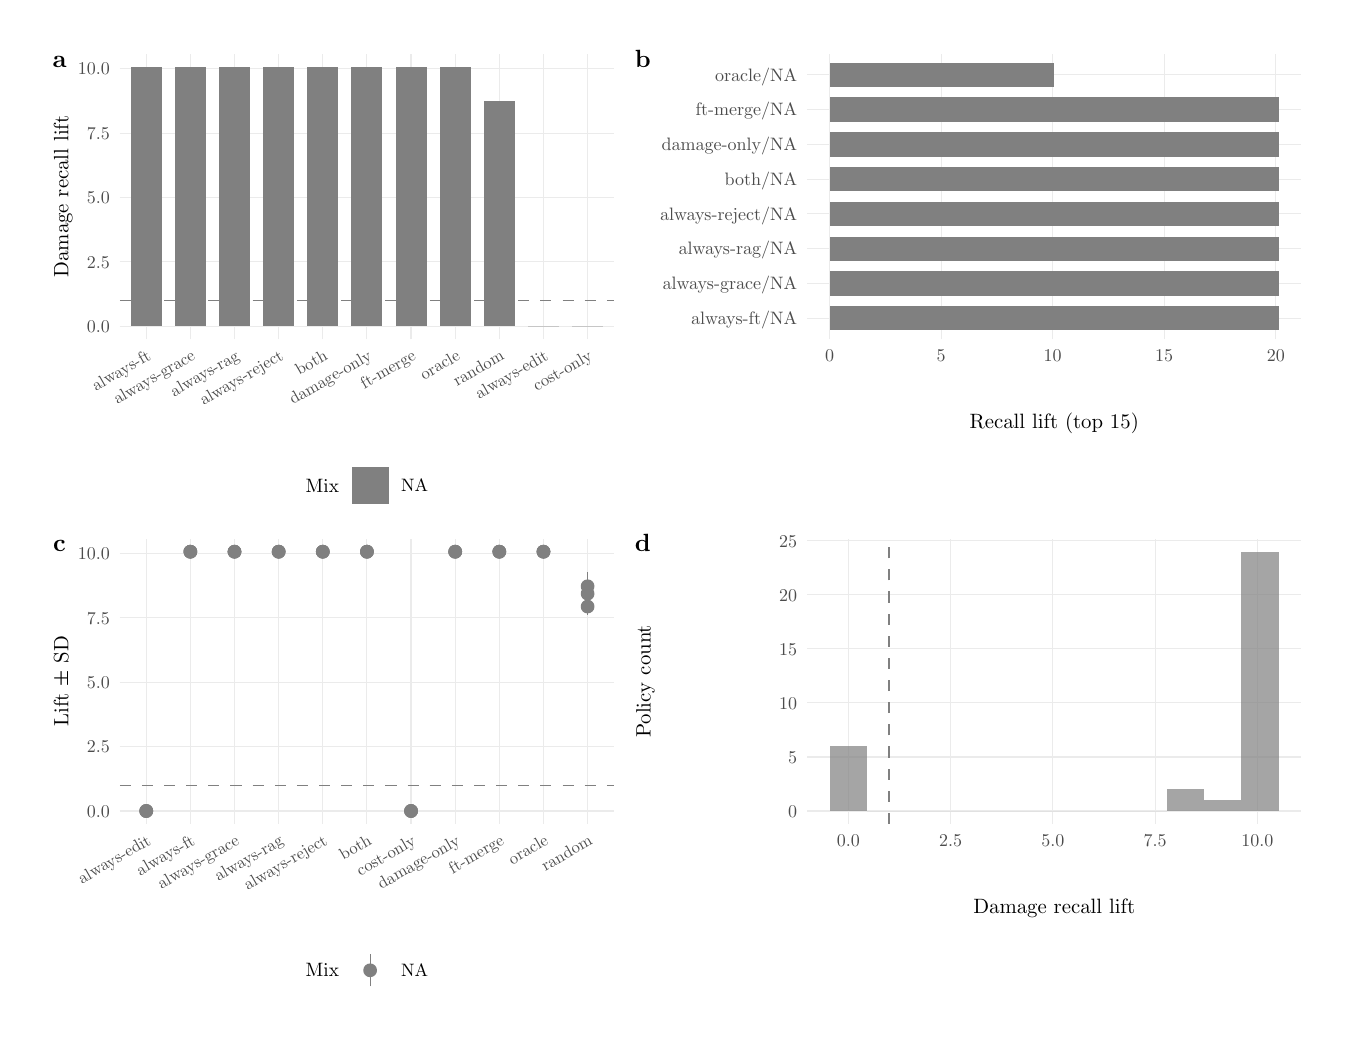
\begin{tikzpicture}[x=1pt,y=1pt]
\definecolor{fillColor}{RGB}{255,255,255}
\path[use as bounding box,fill=fillColor,fill opacity=0.00] (0,0) rectangle (469.75,361.35);
\begin{scope}
\path[clip] (  0.00,  0.00) rectangle (469.75,361.35);
\definecolor{drawColor}{RGB}{255,255,255}
\definecolor{fillColor}{RGB}{255,255,255}

\path[draw=drawColor,line width= 0.6pt,line join=round,line cap=round,fill=fillColor] (  0.00,  0.00) rectangle (469.75,361.35);
\end{scope}
\begin{scope}
\path[clip] (  5.50,180.68) rectangle (215.90,355.85);
\definecolor{fillColor}{RGB}{255,255,255}

\path[fill=fillColor] (  5.50,180.68) rectangle (215.90,355.85);
\end{scope}
\begin{scope}
\path[clip] (215.90,180.68) rectangle (464.25,355.85);
\definecolor{fillColor}{RGB}{255,255,255}

\path[fill=fillColor] (215.90,180.68) rectangle (464.25,355.85);
\end{scope}
\begin{scope}
\path[clip] (  5.50,  5.50) rectangle (215.90,180.67);
\definecolor{fillColor}{RGB}{255,255,255}

\path[fill=fillColor] (  5.50,  5.50) rectangle (215.90,180.67);
\end{scope}
\begin{scope}
\path[clip] (215.90,  5.50) rectangle (464.25,180.67);
\definecolor{fillColor}{RGB}{255,255,255}

\path[fill=fillColor] (215.90,  5.50) rectangle (464.25,180.67);
\end{scope}
\begin{scope}
\path[clip] ( 33.28,248.80) rectangle (211.90,351.85);
\definecolor{drawColor}{gray}{0.92}

\path[draw=drawColor,line width= 0.4pt,line join=round] ( 33.28,253.48) --
	(211.90,253.48);

\path[draw=drawColor,line width= 0.4pt,line join=round] ( 33.28,276.74) --
	(211.90,276.74);

\path[draw=drawColor,line width= 0.4pt,line join=round] ( 33.28,299.99) --
	(211.90,299.99);

\path[draw=drawColor,line width= 0.4pt,line join=round] ( 33.28,323.25) --
	(211.90,323.25);

\path[draw=drawColor,line width= 0.4pt,line join=round] ( 33.28,346.51) --
	(211.90,346.51);

\path[draw=drawColor,line width= 0.4pt,line join=round] ( 42.84,248.80) --
	( 42.84,351.85);

\path[draw=drawColor,line width= 0.4pt,line join=round] ( 58.79,248.80) --
	( 58.79,351.85);

\path[draw=drawColor,line width= 0.4pt,line join=round] ( 74.74,248.80) --
	( 74.74,351.85);

\path[draw=drawColor,line width= 0.4pt,line join=round] ( 90.69,248.80) --
	( 90.69,351.85);

\path[draw=drawColor,line width= 0.4pt,line join=round] (106.64,248.80) --
	(106.64,351.85);

\path[draw=drawColor,line width= 0.4pt,line join=round] (122.59,248.80) --
	(122.59,351.85);

\path[draw=drawColor,line width= 0.4pt,line join=round] (138.53,248.80) --
	(138.53,351.85);

\path[draw=drawColor,line width= 0.4pt,line join=round] (154.48,248.80) --
	(154.48,351.85);

\path[draw=drawColor,line width= 0.4pt,line join=round] (170.43,248.80) --
	(170.43,351.85);

\path[draw=drawColor,line width= 0.4pt,line join=round] (186.38,248.80) --
	(186.38,351.85);

\path[draw=drawColor,line width= 0.4pt,line join=round] (202.33,248.80) --
	(202.33,351.85);
\definecolor{fillColor}{gray}{0.50}

\path[fill=fillColor] (180.80,253.48) rectangle (191.96,253.48);

\path[fill=fillColor] ( 37.26,253.48) rectangle ( 48.43,347.17);

\path[fill=fillColor] ( 53.21,253.48) rectangle ( 64.38,347.17);

\path[fill=fillColor] ( 69.16,253.48) rectangle ( 80.32,347.17);

\path[fill=fillColor] ( 85.11,253.48) rectangle ( 96.27,347.17);

\path[fill=fillColor] (101.06,253.48) rectangle (112.22,347.17);

\path[fill=fillColor] (196.75,253.48) rectangle (207.91,253.48);

\path[fill=fillColor] (117.00,253.48) rectangle (128.17,347.17);

\path[fill=fillColor] (132.95,253.48) rectangle (144.12,347.17);

\path[fill=fillColor] (148.90,253.48) rectangle (160.06,347.17);

\path[fill=fillColor] (164.85,253.48) rectangle (176.01,332.00);

\path[fill=fillColor] (180.80,253.48) rectangle (191.96,253.48);

\path[fill=fillColor] ( 37.26,253.48) rectangle ( 48.43,347.17);

\path[fill=fillColor] ( 53.21,253.48) rectangle ( 64.38,347.17);

\path[fill=fillColor] ( 69.16,253.48) rectangle ( 80.32,347.17);

\path[fill=fillColor] ( 85.11,253.48) rectangle ( 96.27,347.17);

\path[fill=fillColor] (101.06,253.48) rectangle (112.22,347.17);

\path[fill=fillColor] (196.75,253.48) rectangle (207.91,253.48);

\path[fill=fillColor] (117.00,253.48) rectangle (128.17,347.17);

\path[fill=fillColor] (132.95,253.48) rectangle (144.12,347.17);

\path[fill=fillColor] (148.90,253.48) rectangle (160.06,347.17);

\path[fill=fillColor] (164.85,253.48) rectangle (176.01,334.67);

\path[fill=fillColor] (180.80,253.48) rectangle (191.96,253.48);

\path[fill=fillColor] ( 37.26,253.48) rectangle ( 48.43,347.17);

\path[fill=fillColor] ( 53.21,253.48) rectangle ( 64.38,347.17);

\path[fill=fillColor] ( 69.16,253.48) rectangle ( 80.32,347.17);

\path[fill=fillColor] ( 85.11,253.48) rectangle ( 96.27,347.17);

\path[fill=fillColor] (101.06,253.48) rectangle (112.22,347.17);

\path[fill=fillColor] (196.75,253.48) rectangle (207.91,253.48);

\path[fill=fillColor] (117.00,253.48) rectangle (128.17,347.17);

\path[fill=fillColor] (132.95,253.48) rectangle (144.12,347.17);

\path[fill=fillColor] (148.90,253.48) rectangle (160.06,347.17);

\path[fill=fillColor] (164.85,253.48) rectangle (176.01,327.35);
\definecolor{drawColor}{gray}{0.50}

\path[draw=drawColor,line width= 0.5pt,dash pattern=on 4pt off 4pt ,line join=round] ( 33.28,262.78) -- (211.90,262.78);
\end{scope}
\begin{scope}
\path[clip] (  0.00,  0.00) rectangle (469.75,361.35);
\definecolor{drawColor}{gray}{0.30}

\node[text=drawColor,anchor=base east,inner sep=0pt, outer sep=0pt, scale=  0.65] at ( 29.68,251.24) {0.0};

\node[text=drawColor,anchor=base east,inner sep=0pt, outer sep=0pt, scale=  0.65] at ( 29.68,274.50) {2.5};

\node[text=drawColor,anchor=base east,inner sep=0pt, outer sep=0pt, scale=  0.65] at ( 29.68,297.76) {5.0};

\node[text=drawColor,anchor=base east,inner sep=0pt, outer sep=0pt, scale=  0.65] at ( 29.68,321.01) {7.5};

\node[text=drawColor,anchor=base east,inner sep=0pt, outer sep=0pt, scale=  0.65] at ( 29.68,344.27) {10.0};
\end{scope}
\begin{scope}
\path[clip] (  0.00,  0.00) rectangle (469.75,361.35);
\definecolor{drawColor}{gray}{0.30}

\node[text=drawColor,rotate= 30.00,anchor=base east,inner sep=0pt, outer sep=0pt, scale=  0.60] at ( 44.91,241.62) {always-ft};

\node[text=drawColor,rotate= 30.00,anchor=base east,inner sep=0pt, outer sep=0pt, scale=  0.60] at ( 60.86,241.62) {always-grace};

\node[text=drawColor,rotate= 30.00,anchor=base east,inner sep=0pt, outer sep=0pt, scale=  0.60] at ( 76.81,241.62) {always-rag};

\node[text=drawColor,rotate= 30.00,anchor=base east,inner sep=0pt, outer sep=0pt, scale=  0.60] at ( 92.76,241.62) {always-reject};

\node[text=drawColor,rotate= 30.00,anchor=base east,inner sep=0pt, outer sep=0pt, scale=  0.60] at (108.70,241.62) {both};

\node[text=drawColor,rotate= 30.00,anchor=base east,inner sep=0pt, outer sep=0pt, scale=  0.60] at (124.65,241.62) {damage-only};

\node[text=drawColor,rotate= 30.00,anchor=base east,inner sep=0pt, outer sep=0pt, scale=  0.60] at (140.60,241.62) {ft-merge};

\node[text=drawColor,rotate= 30.00,anchor=base east,inner sep=0pt, outer sep=0pt, scale=  0.60] at (156.55,241.62) {oracle};

\node[text=drawColor,rotate= 30.00,anchor=base east,inner sep=0pt, outer sep=0pt, scale=  0.60] at (172.50,241.62) {random};

\node[text=drawColor,rotate= 30.00,anchor=base east,inner sep=0pt, outer sep=0pt, scale=  0.60] at (188.45,241.62) {always-edit};

\node[text=drawColor,rotate= 30.00,anchor=base east,inner sep=0pt, outer sep=0pt, scale=  0.60] at (204.39,241.62) {cost-only};
\end{scope}
\begin{scope}
\path[clip] (  0.00,  0.00) rectangle (469.75,361.35);
\definecolor{drawColor}{RGB}{0,0,0}

\node[text=drawColor,rotate= 90.00,anchor=base,inner sep=0pt, outer sep=0pt, scale=  0.75] at ( 14.67,300.32) {Damage recall lift};
\end{scope}
\begin{scope}
\path[clip] (  0.00,  0.00) rectangle (469.75,361.35);
\definecolor{drawColor}{RGB}{0,0,0}

\node[text=drawColor,anchor=base west,inner sep=0pt, outer sep=0pt, scale=  0.70] at (100.46,193.49) {Mix};
\end{scope}
\begin{scope}
\path[clip] (  0.00,  0.00) rectangle (469.75,361.35);
\definecolor{fillColor}{gray}{0.50}

\path[fill=fillColor] (117.03,189.19) rectangle (130.45,202.61);
\end{scope}
\begin{scope}
\path[clip] (  0.00,  0.00) rectangle (469.75,361.35);
\definecolor{drawColor}{RGB}{0,0,0}

\node[text=drawColor,anchor=base west,inner sep=0pt, outer sep=0pt, scale=  0.65] at (134.97,193.66) {NA};
\end{scope}
\begin{scope}
\path[clip] (  0.00,  0.00) rectangle (469.75,361.35);
\definecolor{drawColor}{RGB}{0,0,0}

\node[text=drawColor,anchor=base,inner sep=0pt, outer sep=0pt, scale=  0.90] at ( 11.52,347.07) {\bfseries a};
\end{scope}
\begin{scope}
\path[clip] (281.63,248.80) rectangle (460.25,351.85);
\definecolor{drawColor}{gray}{0.92}

\path[draw=drawColor,line width= 0.4pt,line join=round] (281.63,256.34) --
	(460.25,256.34);

\path[draw=drawColor,line width= 0.4pt,line join=round] (281.63,268.90) --
	(460.25,268.90);

\path[draw=drawColor,line width= 0.4pt,line join=round] (281.63,281.47) --
	(460.25,281.47);

\path[draw=drawColor,line width= 0.4pt,line join=round] (281.63,294.04) --
	(460.25,294.04);

\path[draw=drawColor,line width= 0.4pt,line join=round] (281.63,306.61) --
	(460.25,306.61);

\path[draw=drawColor,line width= 0.4pt,line join=round] (281.63,319.17) --
	(460.25,319.17);

\path[draw=drawColor,line width= 0.4pt,line join=round] (281.63,331.74) --
	(460.25,331.74);

\path[draw=drawColor,line width= 0.4pt,line join=round] (281.63,344.31) --
	(460.25,344.31);

\path[draw=drawColor,line width= 0.4pt,line join=round] (289.75,248.80) --
	(289.75,351.85);

\path[draw=drawColor,line width= 0.4pt,line join=round] (330.06,248.80) --
	(330.06,351.85);

\path[draw=drawColor,line width= 0.4pt,line join=round] (370.38,248.80) --
	(370.38,351.85);

\path[draw=drawColor,line width= 0.4pt,line join=round] (410.69,248.80) --
	(410.69,351.85);

\path[draw=drawColor,line width= 0.4pt,line join=round] (451.00,248.80) --
	(451.00,351.85);
\definecolor{fillColor}{gray}{0.50}

\path[fill=fillColor] (289.75,251.94) rectangle (370.94,260.73);

\path[fill=fillColor] (289.75,264.51) rectangle (370.94,273.30);

\path[fill=fillColor] (289.75,277.07) rectangle (370.94,285.87);

\path[fill=fillColor] (289.75,289.64) rectangle (370.94,298.44);

\path[fill=fillColor] (289.75,302.21) rectangle (370.94,311.01);

\path[fill=fillColor] (289.75,314.78) rectangle (370.94,323.57);

\path[fill=fillColor] (289.75,327.34) rectangle (370.94,336.14);

\path[fill=fillColor] (289.75,339.91) rectangle (370.94,348.71);

\path[fill=fillColor] (370.94,251.94) rectangle (452.14,260.73);

\path[fill=fillColor] (370.94,264.51) rectangle (452.14,273.30);

\path[fill=fillColor] (370.94,277.07) rectangle (452.14,285.87);

\path[fill=fillColor] (370.94,289.64) rectangle (452.14,298.44);

\path[fill=fillColor] (370.94,302.21) rectangle (452.14,311.01);

\path[fill=fillColor] (370.94,314.78) rectangle (452.14,323.57);

\path[fill=fillColor] (370.94,327.34) rectangle (452.14,336.14);
\end{scope}
\begin{scope}
\path[clip] (  0.00,  0.00) rectangle (469.75,361.35);
\definecolor{drawColor}{gray}{0.30}

\node[text=drawColor,anchor=base east,inner sep=0pt, outer sep=0pt, scale=  0.65] at (278.03,254.10) {always-ft/NA};

\node[text=drawColor,anchor=base east,inner sep=0pt, outer sep=0pt, scale=  0.65] at (278.03,266.67) {always-grace/NA};

\node[text=drawColor,anchor=base east,inner sep=0pt, outer sep=0pt, scale=  0.65] at (278.03,279.23) {always-rag/NA};

\node[text=drawColor,anchor=base east,inner sep=0pt, outer sep=0pt, scale=  0.65] at (278.03,291.80) {always-reject/NA};

\node[text=drawColor,anchor=base east,inner sep=0pt, outer sep=0pt, scale=  0.65] at (278.03,304.37) {both/NA};

\node[text=drawColor,anchor=base east,inner sep=0pt, outer sep=0pt, scale=  0.65] at (278.03,316.94) {damage-only/NA};

\node[text=drawColor,anchor=base east,inner sep=0pt, outer sep=0pt, scale=  0.65] at (278.03,329.50) {ft-merge/NA};

\node[text=drawColor,anchor=base east,inner sep=0pt, outer sep=0pt, scale=  0.65] at (278.03,342.07) {oracle/NA};
\end{scope}
\begin{scope}
\path[clip] (  0.00,  0.00) rectangle (469.75,361.35);
\definecolor{drawColor}{gray}{0.30}

\node[text=drawColor,anchor=base,inner sep=0pt, outer sep=0pt, scale=  0.65] at (289.75,240.72) {0};

\node[text=drawColor,anchor=base,inner sep=0pt, outer sep=0pt, scale=  0.65] at (330.06,240.72) {5};

\node[text=drawColor,anchor=base,inner sep=0pt, outer sep=0pt, scale=  0.65] at (370.38,240.72) {10};

\node[text=drawColor,anchor=base,inner sep=0pt, outer sep=0pt, scale=  0.65] at (410.69,240.72) {15};

\node[text=drawColor,anchor=base,inner sep=0pt, outer sep=0pt, scale=  0.65] at (451.00,240.72) {20};
\end{scope}
\begin{scope}
\path[clip] (  0.00,  0.00) rectangle (469.75,361.35);
\definecolor{drawColor}{RGB}{0,0,0}

\node[text=drawColor,anchor=base,inner sep=0pt, outer sep=0pt, scale=  0.75] at (370.94,216.59) {Recall lift (top 15)};
\end{scope}
\begin{scope}
\path[clip] (  0.00,  0.00) rectangle (469.75,361.35);
\definecolor{drawColor}{RGB}{0,0,0}

\node[text=drawColor,anchor=base,inner sep=0pt, outer sep=0pt, scale=  0.90] at (222.30,347.07) {\bfseries b};
\end{scope}
\begin{scope}
\path[clip] ( 33.28, 73.62) rectangle (211.90,176.68);
\definecolor{drawColor}{gray}{0.92}

\path[draw=drawColor,line width= 0.4pt,line join=round] ( 33.28, 78.30) --
	(211.90, 78.30);

\path[draw=drawColor,line width= 0.4pt,line join=round] ( 33.28,101.56) --
	(211.90,101.56);

\path[draw=drawColor,line width= 0.4pt,line join=round] ( 33.28,124.82) --
	(211.90,124.82);

\path[draw=drawColor,line width= 0.4pt,line join=round] ( 33.28,148.08) --
	(211.90,148.08);

\path[draw=drawColor,line width= 0.4pt,line join=round] ( 33.28,171.33) --
	(211.90,171.33);

\path[draw=drawColor,line width= 0.4pt,line join=round] ( 42.84, 73.62) --
	( 42.84,176.68);

\path[draw=drawColor,line width= 0.4pt,line join=round] ( 58.79, 73.62) --
	( 58.79,176.68);

\path[draw=drawColor,line width= 0.4pt,line join=round] ( 74.74, 73.62) --
	( 74.74,176.68);

\path[draw=drawColor,line width= 0.4pt,line join=round] ( 90.69, 73.62) --
	( 90.69,176.68);

\path[draw=drawColor,line width= 0.4pt,line join=round] (106.64, 73.62) --
	(106.64,176.68);

\path[draw=drawColor,line width= 0.4pt,line join=round] (122.59, 73.62) --
	(122.59,176.68);

\path[draw=drawColor,line width= 0.4pt,line join=round] (138.53, 73.62) --
	(138.53,176.68);

\path[draw=drawColor,line width= 0.4pt,line join=round] (154.48, 73.62) --
	(154.48,176.68);

\path[draw=drawColor,line width= 0.4pt,line join=round] (170.43, 73.62) --
	(170.43,176.68);

\path[draw=drawColor,line width= 0.4pt,line join=round] (186.38, 73.62) --
	(186.38,176.68);

\path[draw=drawColor,line width= 0.4pt,line join=round] (202.33, 73.62) --
	(202.33,176.68);
\definecolor{drawColor}{gray}{0.50}

\path[draw=drawColor,line width= 0.4pt,line join=round] ( 42.84, 78.30) -- ( 42.84, 78.30);

\path[draw=drawColor,line width= 0.4pt,line join=round] ( 58.79,171.99) -- ( 58.79,171.99);

\path[draw=drawColor,line width= 0.4pt,line join=round] ( 74.74,171.99) -- ( 74.74,171.99);

\path[draw=drawColor,line width= 0.4pt,line join=round] ( 90.69,171.99) -- ( 90.69,171.99);

\path[draw=drawColor,line width= 0.4pt,line join=round] (106.64,171.99) -- (106.64,171.99);

\path[draw=drawColor,line width= 0.4pt,line join=round] (122.59,171.99) -- (122.59,171.99);

\path[draw=drawColor,line width= 0.4pt,line join=round] (138.53, 78.30) -- (138.53, 78.30);

\path[draw=drawColor,line width= 0.4pt,line join=round] (154.48,171.99) -- (154.48,171.99);

\path[draw=drawColor,line width= 0.4pt,line join=round] (170.43,171.99) -- (170.43,171.99);

\path[draw=drawColor,line width= 0.4pt,line join=round] (186.38,171.99) -- (186.38,171.99);

\path[draw=drawColor,line width= 0.4pt,line join=round] (202.33,149.10) -- (202.33,164.55);

\path[draw=drawColor,line width= 0.4pt,line join=round] ( 42.84, 78.30) -- ( 42.84, 78.30);

\path[draw=drawColor,line width= 0.4pt,line join=round] ( 58.79,171.99) -- ( 58.79,171.99);

\path[draw=drawColor,line width= 0.4pt,line join=round] ( 74.74,171.99) -- ( 74.74,171.99);

\path[draw=drawColor,line width= 0.4pt,line join=round] ( 90.69,171.99) -- ( 90.69,171.99);

\path[draw=drawColor,line width= 0.4pt,line join=round] (106.64,171.99) -- (106.64,171.99);

\path[draw=drawColor,line width= 0.4pt,line join=round] (122.59,171.99) -- (122.59,171.99);

\path[draw=drawColor,line width= 0.4pt,line join=round] (138.53, 78.30) -- (138.53, 78.30);

\path[draw=drawColor,line width= 0.4pt,line join=round] (154.48,171.99) -- (154.48,171.99);

\path[draw=drawColor,line width= 0.4pt,line join=round] (170.43,171.99) -- (170.43,171.99);

\path[draw=drawColor,line width= 0.4pt,line join=round] (186.38,171.99) -- (186.38,171.99);

\path[draw=drawColor,line width= 0.4pt,line join=round] (202.33,155.37) -- (202.33,163.63);

\path[draw=drawColor,line width= 0.4pt,line join=round] ( 42.84, 78.30) -- ( 42.84, 78.30);

\path[draw=drawColor,line width= 0.4pt,line join=round] ( 58.79,171.99) -- ( 58.79,171.99);

\path[draw=drawColor,line width= 0.4pt,line join=round] ( 74.74,171.99) -- ( 74.74,171.99);

\path[draw=drawColor,line width= 0.4pt,line join=round] ( 90.69,171.99) -- ( 90.69,171.99);

\path[draw=drawColor,line width= 0.4pt,line join=round] (106.64,171.99) -- (106.64,171.99);

\path[draw=drawColor,line width= 0.4pt,line join=round] (122.59,171.99) -- (122.59,171.99);

\path[draw=drawColor,line width= 0.4pt,line join=round] (138.53, 78.30) -- (138.53, 78.30);

\path[draw=drawColor,line width= 0.4pt,line join=round] (154.48,171.99) -- (154.48,171.99);

\path[draw=drawColor,line width= 0.4pt,line join=round] (170.43,171.99) -- (170.43,171.99);

\path[draw=drawColor,line width= 0.4pt,line join=round] (186.38,171.99) -- (186.38,171.99);

\path[draw=drawColor,line width= 0.4pt,line join=round] (202.33,150.37) -- (202.33,153.97);
\definecolor{fillColor}{gray}{0.50}

\path[draw=drawColor,line width= 0.5pt,line join=round,line cap=round,fill=fillColor] ( 42.84, 78.30) circle (  2.23);

\path[draw=drawColor,line width= 0.5pt,line join=round,line cap=round,fill=fillColor] ( 58.79,171.99) circle (  2.23);

\path[draw=drawColor,line width= 0.5pt,line join=round,line cap=round,fill=fillColor] ( 74.74,171.99) circle (  2.23);

\path[draw=drawColor,line width= 0.5pt,line join=round,line cap=round,fill=fillColor] ( 90.69,171.99) circle (  2.23);

\path[draw=drawColor,line width= 0.5pt,line join=round,line cap=round,fill=fillColor] (106.64,171.99) circle (  2.23);

\path[draw=drawColor,line width= 0.5pt,line join=round,line cap=round,fill=fillColor] (122.59,171.99) circle (  2.23);

\path[draw=drawColor,line width= 0.5pt,line join=round,line cap=round,fill=fillColor] (138.53, 78.30) circle (  2.23);

\path[draw=drawColor,line width= 0.5pt,line join=round,line cap=round,fill=fillColor] (154.48,171.99) circle (  2.23);

\path[draw=drawColor,line width= 0.5pt,line join=round,line cap=round,fill=fillColor] (170.43,171.99) circle (  2.23);

\path[draw=drawColor,line width= 0.5pt,line join=round,line cap=round,fill=fillColor] (186.38,171.99) circle (  2.23);

\path[draw=drawColor,line width= 0.5pt,line join=round,line cap=round,fill=fillColor] (202.33,156.82) circle (  2.23);

\path[draw=drawColor,line width= 0.5pt,line join=round,line cap=round,fill=fillColor] ( 42.84, 78.30) circle (  2.23);

\path[draw=drawColor,line width= 0.5pt,line join=round,line cap=round,fill=fillColor] ( 58.79,171.99) circle (  2.23);

\path[draw=drawColor,line width= 0.5pt,line join=round,line cap=round,fill=fillColor] ( 74.74,171.99) circle (  2.23);

\path[draw=drawColor,line width= 0.5pt,line join=round,line cap=round,fill=fillColor] ( 90.69,171.99) circle (  2.23);

\path[draw=drawColor,line width= 0.5pt,line join=round,line cap=round,fill=fillColor] (106.64,171.99) circle (  2.23);

\path[draw=drawColor,line width= 0.5pt,line join=round,line cap=round,fill=fillColor] (122.59,171.99) circle (  2.23);

\path[draw=drawColor,line width= 0.5pt,line join=round,line cap=round,fill=fillColor] (138.53, 78.30) circle (  2.23);

\path[draw=drawColor,line width= 0.5pt,line join=round,line cap=round,fill=fillColor] (154.48,171.99) circle (  2.23);

\path[draw=drawColor,line width= 0.5pt,line join=round,line cap=round,fill=fillColor] (170.43,171.99) circle (  2.23);

\path[draw=drawColor,line width= 0.5pt,line join=round,line cap=round,fill=fillColor] (186.38,171.99) circle (  2.23);

\path[draw=drawColor,line width= 0.5pt,line join=round,line cap=round,fill=fillColor] (202.33,159.50) circle (  2.23);

\path[draw=drawColor,line width= 0.5pt,line join=round,line cap=round,fill=fillColor] ( 42.84, 78.30) circle (  2.23);

\path[draw=drawColor,line width= 0.5pt,line join=round,line cap=round,fill=fillColor] ( 58.79,171.99) circle (  2.23);

\path[draw=drawColor,line width= 0.5pt,line join=round,line cap=round,fill=fillColor] ( 74.74,171.99) circle (  2.23);

\path[draw=drawColor,line width= 0.5pt,line join=round,line cap=round,fill=fillColor] ( 90.69,171.99) circle (  2.23);

\path[draw=drawColor,line width= 0.5pt,line join=round,line cap=round,fill=fillColor] (106.64,171.99) circle (  2.23);

\path[draw=drawColor,line width= 0.5pt,line join=round,line cap=round,fill=fillColor] (122.59,171.99) circle (  2.23);

\path[draw=drawColor,line width= 0.5pt,line join=round,line cap=round,fill=fillColor] (138.53, 78.30) circle (  2.23);

\path[draw=drawColor,line width= 0.5pt,line join=round,line cap=round,fill=fillColor] (154.48,171.99) circle (  2.23);

\path[draw=drawColor,line width= 0.5pt,line join=round,line cap=round,fill=fillColor] (170.43,171.99) circle (  2.23);

\path[draw=drawColor,line width= 0.5pt,line join=round,line cap=round,fill=fillColor] (186.38,171.99) circle (  2.23);

\path[draw=drawColor,line width= 0.5pt,line join=round,line cap=round,fill=fillColor] (202.33,152.17) circle (  2.23);

\path[draw=drawColor,line width= 0.5pt,dash pattern=on 4pt off 4pt ,line join=round] ( 33.28, 87.61) -- (211.90, 87.61);
\end{scope}
\begin{scope}
\path[clip] (  0.00,  0.00) rectangle (469.75,361.35);
\definecolor{drawColor}{gray}{0.30}

\node[text=drawColor,anchor=base east,inner sep=0pt, outer sep=0pt, scale=  0.65] at ( 29.68, 76.07) {0.0};

\node[text=drawColor,anchor=base east,inner sep=0pt, outer sep=0pt, scale=  0.65] at ( 29.68, 99.32) {2.5};

\node[text=drawColor,anchor=base east,inner sep=0pt, outer sep=0pt, scale=  0.65] at ( 29.68,122.58) {5.0};

\node[text=drawColor,anchor=base east,inner sep=0pt, outer sep=0pt, scale=  0.65] at ( 29.68,145.84) {7.5};

\node[text=drawColor,anchor=base east,inner sep=0pt, outer sep=0pt, scale=  0.65] at ( 29.68,169.10) {10.0};
\end{scope}
\begin{scope}
\path[clip] (  0.00,  0.00) rectangle (469.75,361.35);
\definecolor{drawColor}{gray}{0.30}

\node[text=drawColor,rotate= 30.00,anchor=base east,inner sep=0pt, outer sep=0pt, scale=  0.60] at ( 44.91, 66.44) {always-edit};

\node[text=drawColor,rotate= 30.00,anchor=base east,inner sep=0pt, outer sep=0pt, scale=  0.60] at ( 60.86, 66.44) {always-ft};

\node[text=drawColor,rotate= 30.00,anchor=base east,inner sep=0pt, outer sep=0pt, scale=  0.60] at ( 76.81, 66.44) {always-grace};

\node[text=drawColor,rotate= 30.00,anchor=base east,inner sep=0pt, outer sep=0pt, scale=  0.60] at ( 92.76, 66.44) {always-rag};

\node[text=drawColor,rotate= 30.00,anchor=base east,inner sep=0pt, outer sep=0pt, scale=  0.60] at (108.70, 66.44) {always-reject};

\node[text=drawColor,rotate= 30.00,anchor=base east,inner sep=0pt, outer sep=0pt, scale=  0.60] at (124.65, 66.44) {both};

\node[text=drawColor,rotate= 30.00,anchor=base east,inner sep=0pt, outer sep=0pt, scale=  0.60] at (140.60, 66.44) {cost-only};

\node[text=drawColor,rotate= 30.00,anchor=base east,inner sep=0pt, outer sep=0pt, scale=  0.60] at (156.55, 66.44) {damage-only};

\node[text=drawColor,rotate= 30.00,anchor=base east,inner sep=0pt, outer sep=0pt, scale=  0.60] at (172.50, 66.44) {ft-merge};

\node[text=drawColor,rotate= 30.00,anchor=base east,inner sep=0pt, outer sep=0pt, scale=  0.60] at (188.45, 66.44) {oracle};

\node[text=drawColor,rotate= 30.00,anchor=base east,inner sep=0pt, outer sep=0pt, scale=  0.60] at (204.39, 66.44) {random};
\end{scope}
\begin{scope}
\path[clip] (  0.00,  0.00) rectangle (469.75,361.35);
\definecolor{drawColor}{RGB}{0,0,0}

\node[text=drawColor,rotate= 90.00,anchor=base,inner sep=0pt, outer sep=0pt, scale=  0.75] at ( 14.67,125.15) {Lift ± SD};
\end{scope}
\begin{scope}
\path[clip] (  0.00,  0.00) rectangle (469.75,361.35);
\definecolor{drawColor}{RGB}{0,0,0}

\node[text=drawColor,anchor=base west,inner sep=0pt, outer sep=0pt, scale=  0.70] at (100.46, 18.32) {Mix};
\end{scope}
\begin{scope}
\path[clip] (  0.00,  0.00) rectangle (469.75,361.35);
\definecolor{drawColor}{gray}{0.50}

\path[draw=drawColor,line width= 0.4pt,line join=round] (123.74, 14.95) -- (123.74, 26.51);
\definecolor{fillColor}{gray}{0.50}

\path[draw=drawColor,line width= 0.5pt,line join=round,line cap=round,fill=fillColor] (123.74, 20.73) circle (  2.23);
\end{scope}
\begin{scope}
\path[clip] (  0.00,  0.00) rectangle (469.75,361.35);
\definecolor{drawColor}{RGB}{0,0,0}

\node[text=drawColor,anchor=base west,inner sep=0pt, outer sep=0pt, scale=  0.65] at (134.97, 18.49) {NA};
\end{scope}
\begin{scope}
\path[clip] (  0.00,  0.00) rectangle (469.75,361.35);
\definecolor{drawColor}{RGB}{0,0,0}

\node[text=drawColor,anchor=base,inner sep=0pt, outer sep=0pt, scale=  0.90] at ( 11.52,171.90) {\bfseries c};
\end{scope}
\begin{scope}
\path[clip] (281.63, 73.62) rectangle (460.25,176.68);
\definecolor{drawColor}{gray}{0.92}

\path[draw=drawColor,line width= 0.4pt,line join=round] (281.63, 78.30) --
	(460.25, 78.30);

\path[draw=drawColor,line width= 0.4pt,line join=round] (281.63, 97.82) --
	(460.25, 97.82);

\path[draw=drawColor,line width= 0.4pt,line join=round] (281.63,117.34) --
	(460.25,117.34);

\path[draw=drawColor,line width= 0.4pt,line join=round] (281.63,136.86) --
	(460.25,136.86);

\path[draw=drawColor,line width= 0.4pt,line join=round] (281.63,156.38) --
	(460.25,156.38);

\path[draw=drawColor,line width= 0.4pt,line join=round] (281.63,175.89) --
	(460.25,175.89);

\path[draw=drawColor,line width= 0.4pt,line join=round] (296.52, 73.62) --
	(296.52,176.68);

\path[draw=drawColor,line width= 0.4pt,line join=round] (333.47, 73.62) --
	(333.47,176.68);

\path[draw=drawColor,line width= 0.4pt,line join=round] (370.42, 73.62) --
	(370.42,176.68);

\path[draw=drawColor,line width= 0.4pt,line join=round] (407.38, 73.62) --
	(407.38,176.68);

\path[draw=drawColor,line width= 0.4pt,line join=round] (444.33, 73.62) --
	(444.33,176.68);
\definecolor{fillColor}{RGB}{127,127,127}

\path[fill=fillColor,fill opacity=0.70] (289.75, 78.30) rectangle (303.29,101.73);

\path[fill=fillColor,fill opacity=0.70] (303.29, 78.30) rectangle (316.82, 78.30);

\path[fill=fillColor,fill opacity=0.70] (316.82, 78.30) rectangle (330.35, 78.30);

\path[fill=fillColor,fill opacity=0.70] (330.35, 78.30) rectangle (343.88, 78.30);

\path[fill=fillColor,fill opacity=0.70] (343.88, 78.30) rectangle (357.41, 78.30);

\path[fill=fillColor,fill opacity=0.70] (357.41, 78.30) rectangle (370.94, 78.30);

\path[fill=fillColor,fill opacity=0.70] (370.94, 78.30) rectangle (384.48, 78.30);

\path[fill=fillColor,fill opacity=0.70] (384.48, 78.30) rectangle (398.01, 78.30);

\path[fill=fillColor,fill opacity=0.70] (398.01, 78.30) rectangle (411.54, 78.30);

\path[fill=fillColor,fill opacity=0.70] (411.54, 78.30) rectangle (425.07, 86.11);

\path[fill=fillColor,fill opacity=0.70] (425.07, 78.30) rectangle (438.60, 82.21);

\path[fill=fillColor,fill opacity=0.70] (438.60, 78.30) rectangle (452.14,171.99);
\definecolor{drawColor}{gray}{0.50}

\path[draw=drawColor,line width= 0.5pt,dash pattern=on 4pt off 4pt ,line join=round] (311.30, 73.62) -- (311.30,176.68);
\end{scope}
\begin{scope}
\path[clip] (  0.00,  0.00) rectangle (469.75,361.35);
\definecolor{drawColor}{gray}{0.30}

\node[text=drawColor,anchor=base east,inner sep=0pt, outer sep=0pt, scale=  0.65] at (278.03, 76.07) {0};

\node[text=drawColor,anchor=base east,inner sep=0pt, outer sep=0pt, scale=  0.65] at (278.03, 95.58) {5};

\node[text=drawColor,anchor=base east,inner sep=0pt, outer sep=0pt, scale=  0.65] at (278.03,115.10) {10};

\node[text=drawColor,anchor=base east,inner sep=0pt, outer sep=0pt, scale=  0.65] at (278.03,134.62) {15};

\node[text=drawColor,anchor=base east,inner sep=0pt, outer sep=0pt, scale=  0.65] at (278.03,154.14) {20};

\node[text=drawColor,anchor=base east,inner sep=0pt, outer sep=0pt, scale=  0.65] at (278.03,173.66) {25};
\end{scope}
\begin{scope}
\path[clip] (  0.00,  0.00) rectangle (469.75,361.35);
\definecolor{drawColor}{gray}{0.30}

\node[text=drawColor,anchor=base,inner sep=0pt, outer sep=0pt, scale=  0.65] at (296.52, 65.54) {0.0};

\node[text=drawColor,anchor=base,inner sep=0pt, outer sep=0pt, scale=  0.65] at (333.47, 65.54) {2.5};

\node[text=drawColor,anchor=base,inner sep=0pt, outer sep=0pt, scale=  0.65] at (370.42, 65.54) {5.0};

\node[text=drawColor,anchor=base,inner sep=0pt, outer sep=0pt, scale=  0.65] at (407.38, 65.54) {7.5};

\node[text=drawColor,anchor=base,inner sep=0pt, outer sep=0pt, scale=  0.65] at (444.33, 65.54) {10.0};
\end{scope}
\begin{scope}
\path[clip] (  0.00,  0.00) rectangle (469.75,361.35);
\definecolor{drawColor}{RGB}{0,0,0}

\node[text=drawColor,anchor=base,inner sep=0pt, outer sep=0pt, scale=  0.75] at (370.94, 41.41) {Damage recall lift};
\end{scope}
\begin{scope}
\path[clip] (  0.00,  0.00) rectangle (469.75,361.35);
\definecolor{drawColor}{RGB}{0,0,0}

\node[text=drawColor,rotate= 90.00,anchor=base,inner sep=0pt, outer sep=0pt, scale=  0.75] at (225.06,125.15) {Policy count};
\end{scope}
\begin{scope}
\path[clip] (  0.00,  0.00) rectangle (469.75,361.35);
\definecolor{drawColor}{RGB}{0,0,0}

\node[text=drawColor,anchor=base,inner sep=0pt, outer sep=0pt, scale=  0.90] at (222.30,171.90) {\bfseries d};
\end{scope}
\end{tikzpicture}
